\newpage %CV


\pagestyle{empty}


\begin{table}[H]
	\centering
	%	\caption{}
	\label{tab:my-table}
	\resizebox{\textwidth}{!}{%
		\begin{tabular}{lp{0.05cm}p{7.5cm}}
			\centering
			\raisebox{-\totalheight}{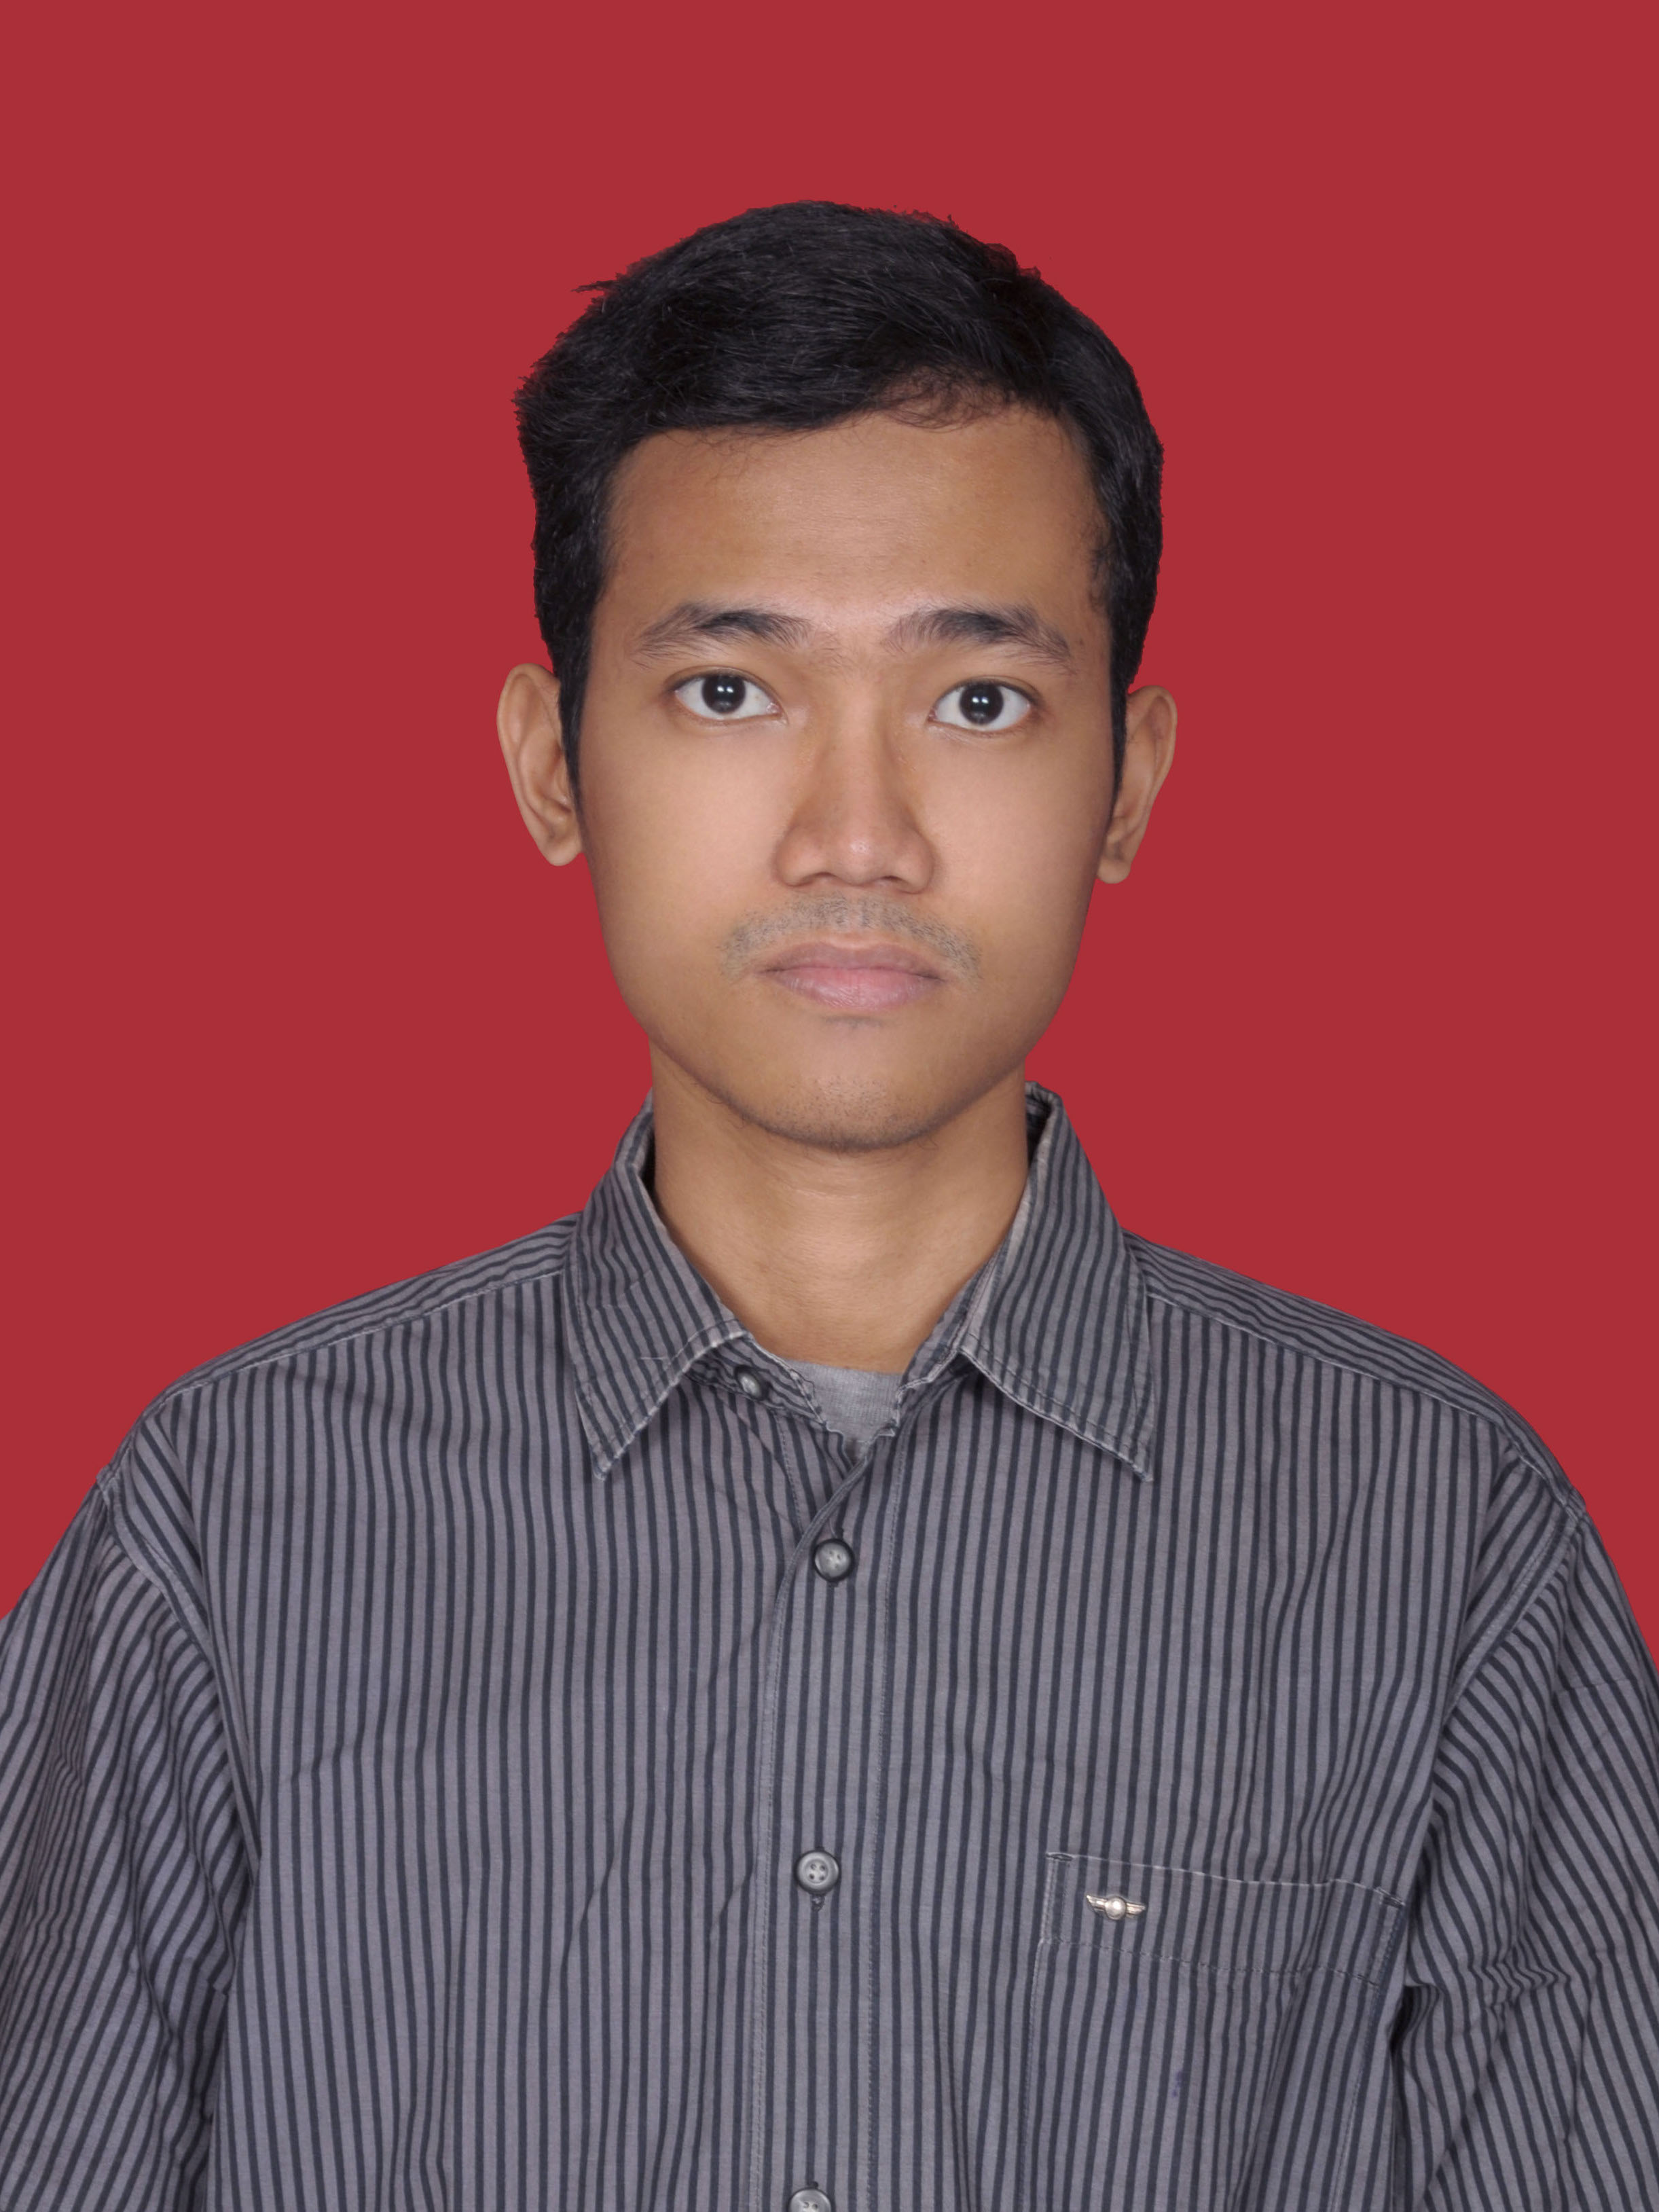
\includegraphics[scale=0.05]{foto_cv_sandy.jpg}} & & \vspace{0.05cm}\LARGE \textbf{RIWAYAT HIDUP}\\
			
		\end{tabular}
	}
\end{table}

\vspace{1cm}
\noindent \textbf{IDENTITAS DIRI}
\vspace{0.2cm}


\begin{table}[H]
	%	\caption{}
	\label{tab:my-table}
	%	\resizebox{\textwidth}{!}
\end{table}


\vspace{8cm}
\noindent \textbf{PENDIDIKAN FORMAL}
\vspace{0.2cm}

% Please add the following required packages to your document preamble:
% \usepackage{graphicx}
\begin{table}[H]
		\centering
	%	\caption{}
	\label{tab:my-table}
	%	\resizebox{\textwidth}{!}{%
	\begin{longtable}{|c|l|p{7.5cm}|}
		\hline
		\textbf{Tahun} & \multicolumn{1}{c|}{\textbf{Pendidikan}} & \multicolumn{1}{c|}{\textbf{Institusi}} \\ \hline
		1999 & TK & TK Aisyiah 37 Jakarta \\ \hline
		2005 & SD & SD N Menteng 02 Jakarta\\ \hline
		2008 & SMP & SMP Negeri 216 Jakarta \\ \hline
		2011 & SMA & SMA Negeri 28 Jakarta \\ \hline
		2015 & S1   Teknik Elektro & Universitas Gunadarma         \\ \hline
		2016 & S2  Teknik Elektro & Universitas Gunadarma  \\ \hline
		------ & S3   Teknologi Informasi & Universitas Gunadarma \\ \hline
	\end{longtable}%
	%	}
		\centering	
\end{table}

%\newpage
\vspace{0.5cm}
\noindent \textbf{PENGALAMAN DILUAR PENDIDIKAN FORMAL}
\vspace{0.2cm}


% Please add the following required packages to your document preamble:
% \usepackage{graphicx}
\begin{table}[H]
		\centering
	%	\caption{}
	%	\label{tab:my-table}
	%	\resizebox{\textwidth}{!}{%
	\begin{tabular}{|l|p{11.5cm}|}
		\hline
		\multicolumn{1}{|c|}{\textbf{Tahun}} & \multicolumn{1}{c|}{\textbf{Jabatan}}                      \\ \hline
		2016      & \textit{Linneaus Palme Schoolarship Swedia - Student Exchange}  \\ \hline
		2017 -      &  Dosen Tetap Universitas Gunadarma \\ \hline
		2017 -      &  Reviewer Nasional Program Kreatifitas Mahasiswa - Kemdikbud \\ \hline
		2017 -      &  Pilot Drone Licences Asosiasi Pilot Drone Indonesia  - Kemenhub\\ \hline
	\end{tabular}%
	%	}
		\centering
\end{table}


%\newpage
\vspace{0.5cm}
\noindent \textbf{PUBLIKASI ILMIAH}
\vspace{0.2cm}


% Please add the following required packages to your document preamble:
% \usepackage{graphicx}
\begin{table}[H]
	%	\centering
	%	\caption{}
	%	\label{tab:my-table}
	%	\resizebox{\textwidth}{!}{%
	\begin{tabular}{|c|p{6cm}|p{5.7cm}|}
		\hline
		\textbf{Tahun} &
		\multicolumn{1}{c|}{\textbf{Penulis-Judul}} &
		\multicolumn{1}{c|}{\textbf{Keterangan}} \\ \hline
		2020 & Sandy Suryo Prayogo, Tubagus Maulana Kusuma -  Analisis Sensitivitas Video MPEG-4 berdasarkan Struktur Frame Pada Transmisi DVB-T
 & Jurnal Ilmiah Informatika Komputer 25 (2), 86-97 , Universitas Gunadarma\\ \hline
		2023 &  -  & \textit{-} \\ \hline
		2023 &  -  & \textit{-} \\ \hline

	\end{tabular}%
	%	}
\end{table}


 



